\documentclass[11pt]{article}
\usepackage[utf8]{inputenc}
\usepackage[T1]{fontenc}
\usepackage[spanish]{babel}
\usepackage{amsmath}
\usepackage{booktabs}
\usepackage{graphicx}
\usepackage{float}
\usepackage{geometry}
\usepackage{array}
\geometry{margin=2.5cm}
\setlength{\parskip}{0.65em}
\setlength{\parindent}{0pt}
\title{Informe de resultados: Desempleo macro}
\author{FinPUC}
\date{}
\begin{document}
\maketitle

\section{Análisis de resultados fuera de muestra}
Esta iteración evalúa la view \textit{Desempleo macro} dentro de la misma arquitectura de tres horizontes y ventanas móviles utilizada en la validación robustecida. La etapa de calibración no vuelve a competir contra otras familias de views; en cambio, fija la familia analizada y calibra secuencialmente su estructura interna hasta congelar la configuración final: familia unemployment, lookback 252 días, long/short 20, ponderación equal, q\_scale=1.5, confianza=50\%, $\tau$=0.200.
En promedio, la mejora porcentual de Sharpe frente a Markowitz fue 2.0\%, con una fracción recomendada media de 40.0\% sobre los cruces escenario-perfil. La señal produce una dinámica operacionalmente estable: bajo turnover, alta diversificación efectiva y una concentración sectorial acotada.
\begin{table}[H]
\centering
\resizebox{\textwidth}{!}{%
\begin{tabular}{lrrrrrrr}
\toprule
Escenario & Perfil & Sharpe BL & Sharpe MK & Mejora Sharpe & DD BL & DD MK & \% ventanas recomendado \\
\midrule
sin\_pandemia & Muy conservador & 1.738 & 1.736 & 0.2\% & -10.2\% & -10.3\% & 100.0\% \\
sin\_pandemia & Conservador & 1.718 & 1.728 & -0.6\% & -10.1\% & -11.0\% & 0.0\% \\
sin\_pandemia & Neutro & 1.664 & 1.747 & -4.8\% & -10.2\% & -13.0\% & 0.0\% \\
sin\_pandemia & Arriesgado & 1.562 & 1.513 & 3.2\% & -12.1\% & -18.2\% & 100.0\% \\
sin\_pandemia & Muy arriesgado & 1.154 & 1.198 & -3.7\% & -21.1\% & -26.5\% & 0.0\% \\
con\_pandemia & Muy conservador & 1.625 & 1.699 & -4.4\% & -9.1\% & -9.0\% & 0.0\% \\
con\_pandemia & Conservador & 1.638 & 1.749 & -6.5\% & -9.2\% & -9.0\% & 0.0\% \\
con\_pandemia & Neutro & 1.660 & 1.773 & -6.0\% & -9.4\% & -10.9\% & 25.0\% \\
con\_pandemia & Arriesgado & 1.644 & 1.391 & 19.9\% & -11.1\% & -18.7\% & 75.0\% \\
con\_pandemia & Muy arriesgado & 1.119 & 0.933 & 23.1\% & -22.8\% & -27.6\% & 100.0\% \\
\bottomrule
\end{tabular}
}
\caption{Comparación fuera de muestra en horizonte limpio para Desempleo macro.}
\label{tab:desempleo_macro:resultados_oos}
\end{table}

\begin{figure}[H]
\centering
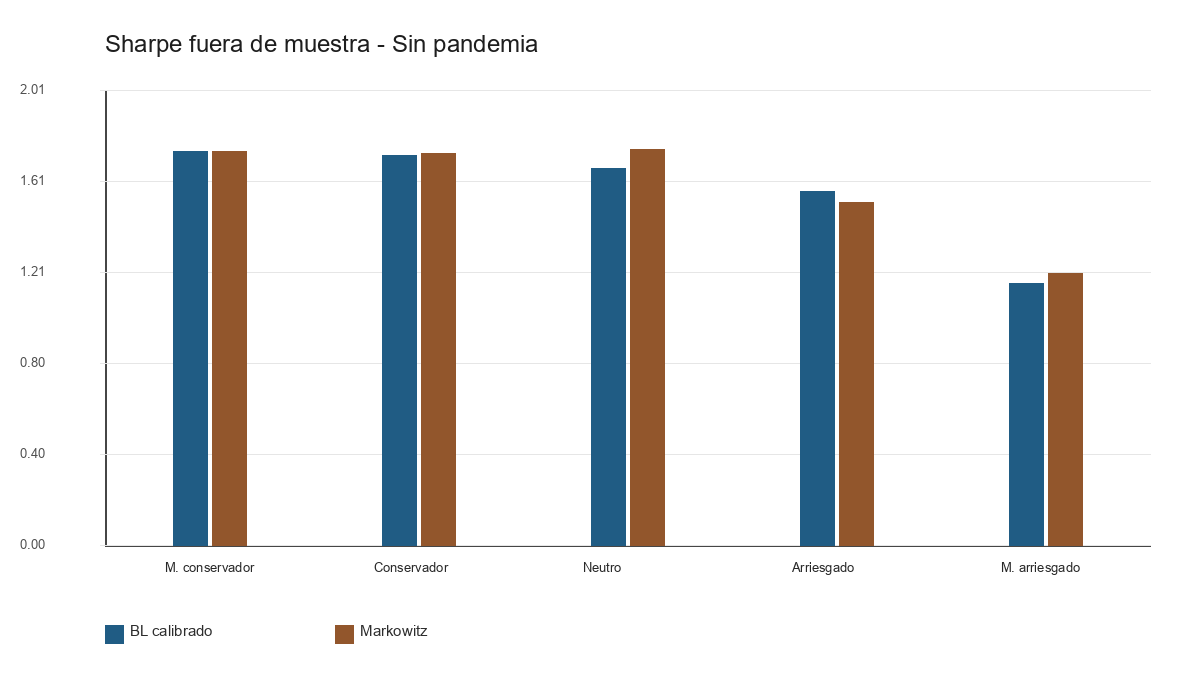
\includegraphics[width=0.92\textwidth]{figuras/sharpe_sin_pandemia.png}
\caption{Sharpe fuera de muestra sin pandemia para Desempleo macro.}
\label{fig:desempleo_macro:sharpe_sin}
\end{figure}
\begin{figure}[H]
\centering
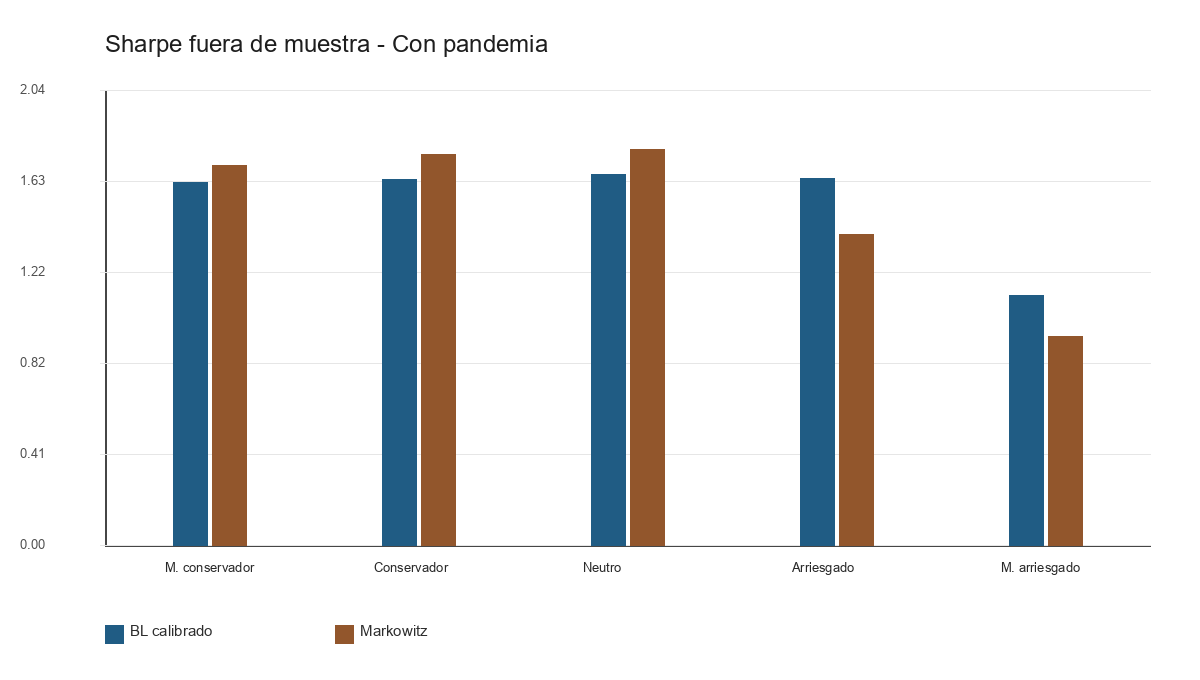
\includegraphics[width=0.92\textwidth]{figuras/sharpe_con_pandemia.png}
\caption{Sharpe fuera de muestra con pandemia para Desempleo macro.}
\label{fig:desempleo_macro:sharpe_con}
\end{figure}

\section{Resultados de la dinámica de portafolio}
La dinámica del portafolio se analiza como una condición de implementabilidad. Un modelo puede mejorar el Sharpe fuera de muestra, pero si lo hace mediante rotación excesiva, concentración sectorial o inestabilidad de pesos, su recomendación debe ser tratada como condicional.
\begin{table}[H]
\centering
\resizebox{\textwidth}{!}{%
\begin{tabular}{lrrrrrr}
\toprule
Escenario & Perfil & Turnover & Turn. >20\% & N efectivo & HHI sector & Peso sector líder \\
\midrule
sin\_pandemia & Muy conservador & 7.0\% & 0.0\% & 221.21 & 0.147 & 27.5\% \\
sin\_pandemia & Conservador & 7.0\% & 0.0\% & 233.51 & 0.144 & 27.2\% \\
sin\_pandemia & Neutro & 6.9\% & 0.0\% & 271.13 & 0.137 & 26.2\% \\
sin\_pandemia & Arriesgado & 6.9\% & 0.0\% & 360.45 & 0.124 & 21.8\% \\
sin\_pandemia & Muy arriesgado & 9.2\% & 0.0\% & 163.27 & 0.178 & 32.1\% \\
con\_pandemia & Muy conservador & 6.3\% & 0.0\% & 112.55 & 0.169 & 25.7\% \\
con\_pandemia & Conservador & 6.2\% & 0.0\% & 118.08 & 0.166 & 25.0\% \\
con\_pandemia & Neutro & 6.4\% & 0.0\% & 136.34 & 0.158 & 23.5\% \\
con\_pandemia & Arriesgado & 7.0\% & 0.0\% & 205.71 & 0.135 & 20.1\% \\
con\_pandemia & Muy arriesgado & 9.9\% & 0.0\% & 120.96 & 0.214 & 37.9\% \\
\bottomrule
\end{tabular}
}
\caption{Dinámica de portafolio de Black-Litterman calibrado para Desempleo macro.}
\label{tab:desempleo_macro:dinamica}
\end{table}

\begin{figure}[H]
\centering
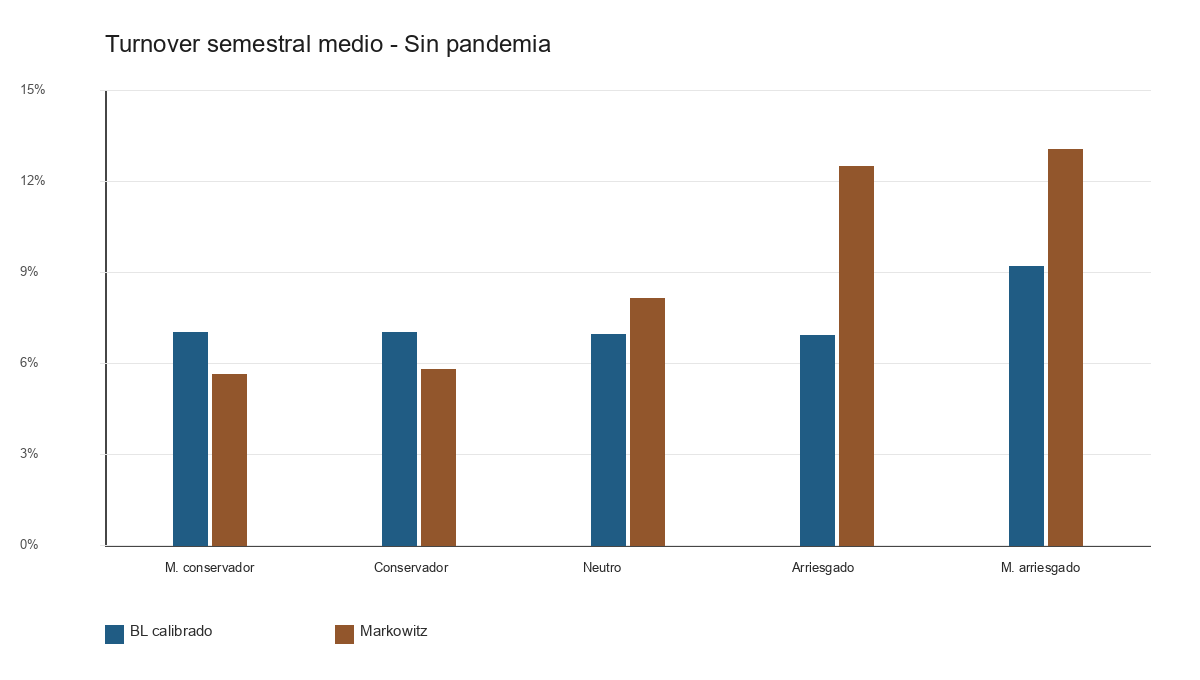
\includegraphics[width=0.92\textwidth]{figuras/turnover_sin_pandemia.png}
\caption{Turnover semestral medio sin pandemia para Desempleo macro.}
\label{fig:desempleo_macro:turnover_sin}
\end{figure}
\begin{figure}[H]
\centering
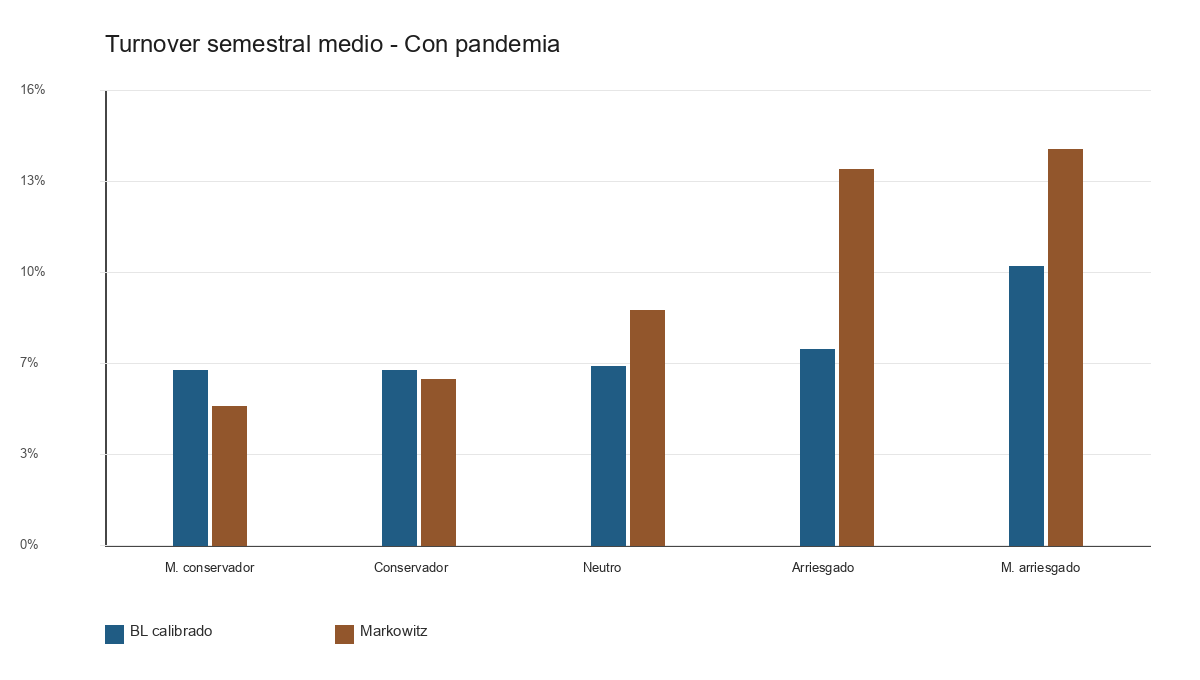
\includegraphics[width=0.92\textwidth]{figuras/turnover_con_pandemia.png}
\caption{Turnover semestral medio con pandemia para Desempleo macro.}
\label{fig:desempleo_macro:turnover_con}
\end{figure}

\section{Evaluación Económica Monte Carlo P4 en Horizonte Limpio}
La simulación Monte Carlo P4 se ejecuta únicamente en el Horizonte 3. Por diseño, la utilidad de la empresa es un resultado ex-post asociado al saldo administrado activo y no entra en el optimizador de portafolios. En esta iteración se reportan explícitamente la probabilidad de aceptación inicial, la probabilidad de aceptación del rebalanceo, la probabilidad semanal de abandono y el número de clientes activos al final de las 260 semanas.
\begin{table}[H]
\centering
\resizebox{\textwidth}{!}{%
\begin{tabular}{lrrrrrrrr}
\toprule
Escenario & Perfil & Riqueza & Utilidad empresa & P acepta inicial & P acepta reb. & P abandono semanal & Clientes iniciales & Clientes finales \\
\midrule
sin\_pandemia & Muy conservador & 1.698 & 34 & 99.0\% & 99.0\% & 0.7\% & 1986 & 716 \\
sin\_pandemia & Conservador & 2.489 & 73 & 97.0\% & 97.0\% & 0.1\% & 1925 & 1625 \\
sin\_pandemia & Neutro & 2.300 & 67 & 78.9\% & 78.9\% & 0.0\% & 1580 & 1571 \\
sin\_pandemia & Arriesgado & 1.250 & 13 & 15.2\% & 15.2\% & 0.0\% & 317 & 317 \\
sin\_pandemia & Muy arriesgado & 1.077 & 4 & 3.8\% & 3.8\% & 0.0\% & 82 & 82 \\
con\_pandemia & Muy conservador & 1.564 & 31 & 98.1\% & 98.1\% & 0.7\% & 1961 & 708 \\
con\_pandemia & Conservador & 2.243 & 68 & 95.1\% & 95.1\% & 0.1\% & 1910 & 1626 \\
con\_pandemia & Neutro & 2.130 & 61 & 73.8\% & 73.8\% & 0.0\% & 1486 & 1478 \\
con\_pandemia & Arriesgado & 1.249 & 13 & 15.5\% & 15.5\% & 0.0\% & 305 & 305 \\
con\_pandemia & Muy arriesgado & 1.110 & 5 & 4.8\% & 4.8\% & 0.0\% & 104 & 104 \\
\bottomrule
\end{tabular}
}
\caption{Resultados P4 y comportamiento de clientes para Desempleo macro.}
\label{tab:desempleo_macro:p4}
\end{table}

\begin{figure}[H]
\centering
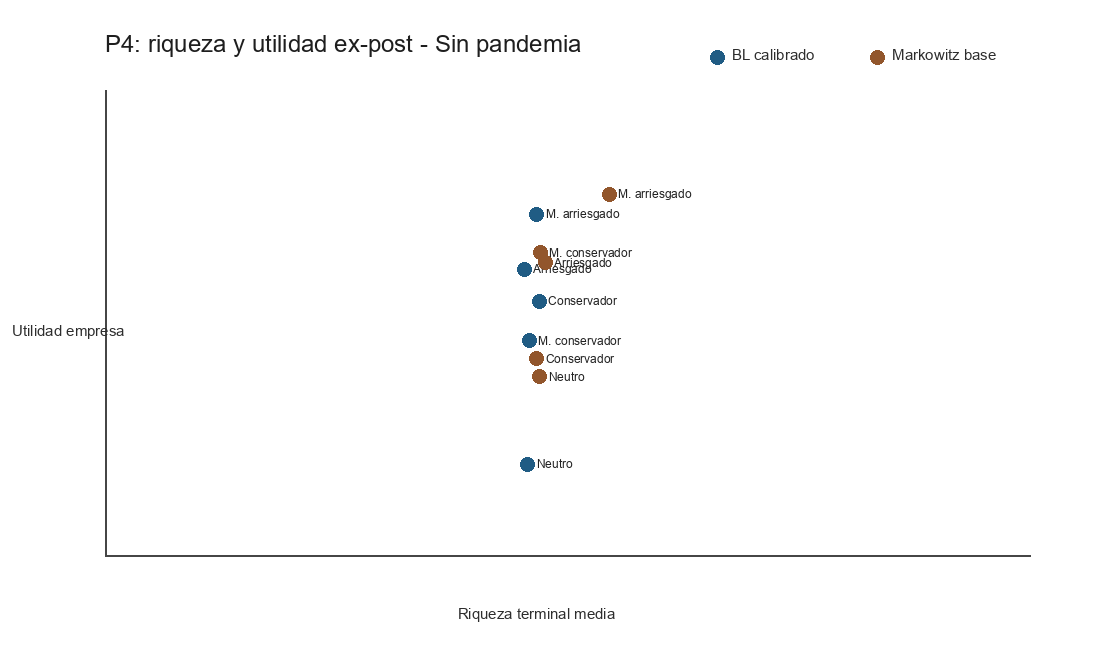
\includegraphics[width=0.88\textwidth]{figuras/p4_riqueza_utilidad_sin_pandemia.png}
\caption{Relación entre riqueza terminal y utilidad ex-post sin pandemia para Desempleo macro.}
\label{fig:desempleo_macro:p4_sin}
\end{figure}
\begin{figure}[H]
\centering
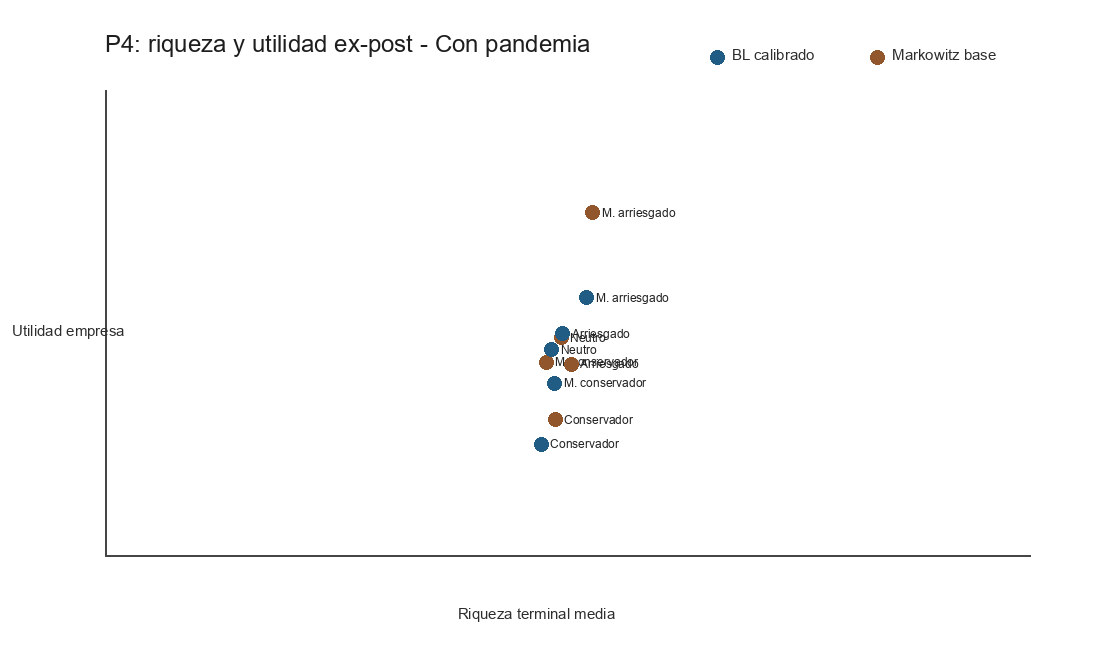
\includegraphics[width=0.88\textwidth]{figuras/p4_riqueza_utilidad_con_pandemia.png}
\caption{Relación entre riqueza terminal y utilidad ex-post con pandemia para Desempleo macro.}
\label{fig:desempleo_macro:p4_con}
\end{figure}

\section{Discusión de Robustez}
El contraste con y sin pandemia permite separar rendimiento promedio de resiliencia. Para Desempleo macro, la lectura relevante no es si Black-Litterman domina todos los cruces, sino si la señal conserva un balance defendible entre Sharpe, drawdown, estabilidad de composición y comportamiento económico de los clientes. Los perfiles con mejora financiera pero rotación alta deben considerarse de mayor costo operativo y menor robustez implementable.

\section{Conclusiones}
\begin{table}[H]
\centering
\resizebox{\textwidth}{!}{%
\begin{tabular}{lrrrrrr}
\toprule
Perfil & Mejora Sharpe media & \% recomendado & Turnover & HHI sector & N efectivo & Lectura \\
\midrule
Muy conservador & -2.1\% & 50.0\% & 6.6\% & 0.158 & 166.88 & Recomendable \\
Conservador & -3.5\% & 0.0\% & 6.6\% & 0.155 & 175.79 & No preferente \\
Neutro & -5.4\% & 12.5\% & 6.6\% & 0.147 & 203.73 & No preferente \\
Arriesgado & 11.6\% & 87.5\% & 6.9\% & 0.130 & 283.08 & Recomendable \\
Muy arriesgado & 9.7\% & 50.0\% & 9.5\% & 0.196 & 142.11 & Recomendable \\
\bottomrule
\end{tabular}
}
\caption{Recomendación segmentada para Desempleo macro.}
\label{tab:desempleo_macro:conclusiones}
\end{table}

En síntesis, la recomendación metodológica de esta view debe leerse por perfil de riesgo y no como una regla única. Cuando la mejora de Sharpe se sostiene junto con baja rotación y baja concentración, la señal es apta para recomendación directa. Cuando la mejora viene acompañada de turnover elevado o concentración sectorial, su uso debe limitarse a perfiles que toleren cambios frecuentes y mayor exposición táctica.
\end{document}